\documentclass[12pt, a4paper]{article}

\usepackage[utf8]{inputenc}
\usepackage[T1]{fontenc}
\usepackage[francais]{babel}
\usepackage[top=2cm, bottom=2cm, left=1.2cm, right=2cm]{geometry}
\usepackage{verbatim}
\usepackage{graphicx}
\usepackage{listings}
\lstset{
%upquote=true,
columns=flexible,
basicstyle=\ttfamily,}

\title{Projet IHM - Rapport 3 - RICM4}
\author{\bsc{Fréby} Rodolphe - \bsc{Barbier} Jérome - \bsc{Husson} Augustin - \bsc{Labat} Paul}
\date{\today}



\begin{document}
\maketitle
\tableofcontents
\newpage

\section{Introduction}
Voici le 3ème et dernier rapport du projet d'IHM. Il a pour objectif de présenter les critères de Scapin et Bastien que notre prototype respecte, après une description de ces fonctionnalités.

\section{Organisation de la fenêtre}

Tout d'abord, la hiérarchie des objets de l'interface est la suivante :
ici faire le dessin de la hiérarchie pour la fenêtre.

Ensuite, l'organisation des éléments dans la fenêtre est la suivante :

\begin{figure}[h]
\begin{center}
   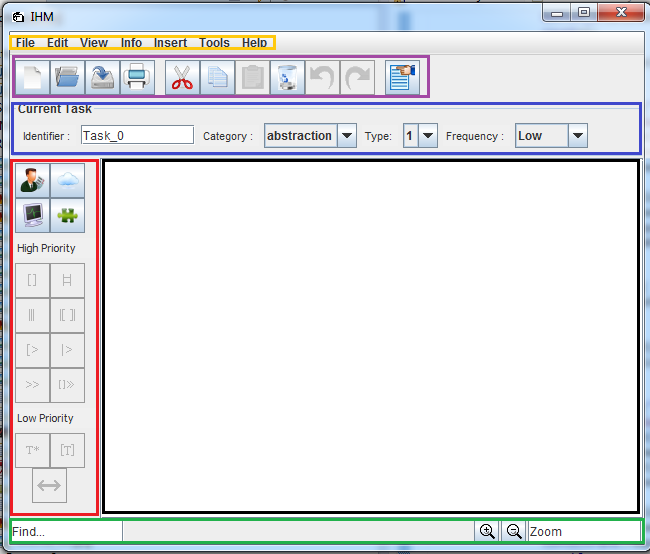
\includegraphics[scale = 0.7]{interface.png}
	\caption{Notre interface}
	\end{center}
\end{figure}

\begin{itemize}
\item [*]La zone jaune représente les différents menu avec la grande majorité des options spécifiques, tel que la sauvegarde en jpg, l'accès à l'aide, etc... 
\item [*]La zone violette regroupe les différents outils de manipulation rapide de fichier. Ils sont triés par sous groupe en fonction de leur utilisation. 
\item [*]La zone suivante, en bleu, permet de voir en temps réel les informations du nœud sélectionné (le nœud courant), et de les modifier au besoin. 
\item [*]La zone noire représente elle la zone de travail dans laquelle l'arbre s'affiche. 
\item [*]En rouge, il s'agit de la zone de travail sur les nœuds, pour leur création, ou les opérateurs d'association. 
\item [*]Enfin, la zone verte permet à l'utilisateur d'utiliser la recherche d'un nœud dans l'arbre, et la fonctionnalité zoom.
\end{itemize}

\section{spécifications techniques}

\subsection{Nos choix}

En premier lieu, nous avons décider d'enlever un certain nombre de boutons de la fenêtre. Pour commencer, nous avons jugé que la sauvegarde en temps que \emph{JPG} n'est pas de première nécessité et n'est pas utiliser souvent. De même, nous avons considéré qu'un utilisateur utilisera plus souvent les options de copiage et de coupage par \emph{SubTree}, donc nous avons retiré de la barre la fonction \emph{Cut}. Toujours en suivant ce raisonnement, pour nous le \emph{check model structur} et \emph{insert mode} ne sont pas de première importance, comme les 4 boutons de travaux sur la hauteur des arbres. Nous estimions également que le zoom n'était pas agréable à utiliser, nous avons préférer prendre un système ou l'utilisateur aurait toujours le choix de la valeur de zoom, ou bien mettre un zoom par un pas prédéfini, et placer les options en bas à droite de l'écran de manière plus discrète. Nous avons définitivement enlever les options de modification du texte. Elles sont dans notre façon de voir les choses par clique droit / propriété ou par clique sur le bouton propriété d'un nœud (En effet, comme quand nous utilisons un document word, la majorité de nos travaux n'ont pas vocation à fournir un rapport ou un produit final, seulement des documents succins. L’intérêt de la modification de la police et de la taille de caractère ne nous semble pas la plus importante).\\


Nous avons par la suite supprimer \emph{l'overview}, qui pour nous ne présente aucun intérêt. Un utilisateur préfèrera selon nous se déplacer sur son espace de travail plutôt que de regarder dans un \emph{overview} trop petit pour fournir des informations pertinentes. Nous avons garder la zone de modification rapide d'un nœud, en apportant une modification. Nous avons créé une liste déroulante pour le type. En effet, ce champ attend toujours une valeur précise, plutôt que de la faire rentré par un utilisateur qui pourrait se tromper, nous fournissons la liste des types que l'utilisateur choisi. Nous avons également enlevé la plateforme, qui est disponible dans les paramètres complets accessible comme expliqué précédemment.\\



Pour le bandeau de gauche, nous avons voulu le rendre plus visible, car celui-ci nous paraissait écrasé. Pour cela, nous avons décider de faire deux colonnes de boutons. Nous les avons tous garder, car nous estimons qu'ils sont tous important. Nous avons choisi en revanche de fournir des infobulles plus conséquentes, afin de mieux aider un utilisateur novice à comprendre les différentes fonctions.\\


Afin de rendre le logiciel plus ``jeune'', nous avons décider de mettre de nouvelles icônes. En particulier, la sauvegarde est désormais un disque dur avec une flèche, les disquettes ayant disparues de nos espaces de travail. Nous avons ajouté une fonction de recherche, car dans les grands arbres, il peut être difficile de s'y retrouver. Pouvoir chercher un nœud en particulier nous est important. Nous avons placé ce bouton de manière discrète en bas à gauche.\\


Afin de moins surcharger les menus, nous avons décider de regrouper les différentes options de sauvegarde dans un même onglet, nommé \emph{Save as}. Nous avons ajouté un bandeau \emph{Help}, proposant un tutoriel, également proposé à la première ouverture du logiciel, et une section aide avec possibilité d'effectuer une recherche dedans.\\


Nous avons ré implémenté la totalité des options, ainsi que les raccourcis, en ajoutant les raccourcis MacOS avec la touche \emph{Command} (comme spécifié plus tard). Une demande de confirmation pour quitter le logiciel est demandé, afin de s'assurer que l'utilisateur ne quittera pas par erreur sans enregistrer son travail. De même, nous avons placé une taille de fenêtre minimal (inséré la valeur créée ici).

Si il manque des choses selon vous, à completer....
\subsection{Raccourcis clavier}

Un large choix de raccourcis clavier ont été ajoutés sur le logiciels, fonctionnant sous Windows, Linux ou MacOS (Paul si tu peux préciser la version)

\begin{tabular}{| c | c | c |}
\hline
Fonction & Raccourcis avec CTRL & Raccourcis avec Command \\ \hline
Trouver & CTRL + F & Command + F \\ \hline
Arbre prioritaire & CTRL + T & Command + T \\ \hline
Copier & CTRL + C & Command + C \\ \hline
Coller  & CTRL + V & Command + V \\ \hline
Couper & CTRL + X & Command + X \\ \hline
Nouveau niveau & CTRL + L & Command + L \\ \hline
Fold / Unfold sous arbre & CTRL + H & Command + H \\ \hline
Unfold tout & CTRL + U & Command + U \\ \hline
Retour avant & CTRL + Z & Command + Z \\ \hline
Retour arrière & CTRL + Y & Command + Y \\ \hline
Description informelle à description formelle & CTRL + D & Command + D \\ \hline
Imprimer & CTRL + P & Command + P \\ \hline
Reachablelity analysis  & CTRL + A & Command + A \\ \hline
Ouvrir & CTRL + O & Command + O \\ \hline
Nouveau & CTRL + N & Command + N \\ \hline
Coller SubTree & CTRL + SHIFT + V & Command + SHIFT + V \\ \hline
Copier SubTree & CTRL + SHIFT + C & Command + SHIFT + C \\ \hline
Ouvrir CTT en tant que XML  & CTRL + SHIFT + O & Command + SHIFT + O \\ \hline
Enregistrer en tant que... & CTRL + SHIFT + S & Command + SHIFT + S \\ \hline
Imprimer en plusieurs pages & CTRL + SHIFT + P & Command + SHIFT + P \\ \hline
Model Filter & CTRL + SHIFT + F & Command + SHIFT + F \\ \hline
Supprimer & Supprimer & / \\ \hline
Inserer sous arbre par fichier & Insert & / \\ \hline
Vérification de la structure du modèle & F7 & / \\ \hline
Start task model simulator & F4 & / \\ \hline
\end{tabular}

\section{Les critères de Scapin et Bastien et notre interface}

\section{Fonctionnalités non disponibles}

Notre prototype n'est qu'une interface, et la création d'un arbre n'est donc pas réalisable. La plupart des options ne font qu'ouvrir des pop-up. La sauvegarde et l'ouverture de fichier ne fonctionne pas également.
\end{document}